\modeCorrection

%%%% début de la page
\renewcommand{\thesection}{\textcolor{red}{Partie \Roman{section} -}}
\renewcommand{\thesubsection}{\textcolor{red}{\Roman{section}.\arabic{subsection}}}
\renewcommand{\thesubsubsection}{\textcolor{red}{\Roman{section}.\arabic{subsection}.\alph{subsubsection}}}

\setcounter{section}{0}
\setcounter{document}{0}
\sndEnTeteTPDix

\nomPrenomClasse

\begin{center}
\begin{mdframed}[style=titr, leftmargin=60pt, rightmargin=60pt, innertopmargin=7pt, innerbottommargin=7pt, innerrightmargin=8pt, innerleftmargin=8pt]

\begin{center}
\large{\textbf{TP 10 : L'apparition d'un arc-en-ciel
}}
\end{center}
\end{mdframed}
\end{center}

\begin{tableauCompetences}
    \hline
    APP & Exploiter un spectre d'émission & & & & \\   
    \hline 
    REA & Connaître et exploiter les lois de Snell-Descartes & & & & \\
    \hline 
    COM & Rendre compte de façon écrite & & & & 
\end{tableauCompetences}


%%%% objectifs
\begin{tcolorbox}[colback=blue!5!white,colframe=blue!75!black,title=Objectifs de la séance :]
\begin{itemize}
    \item Décrire et expliquer qualitativement le phénomène de dispersion de la lumière par un prisme ;
    \item Exploiter des spectres d'émission obtenus à l'aide d'un système dispersif ;
\end{itemize}
\end{tcolorbox}

%%%% Consignes
\begin{tcolorbox}[colback=red!5!white,colframe=red!75!black,title= Consignes :]
\begin{itemize}
    \item Rédiger un compte-rendu individuel ;
    \item Interdiction de se déplacer dans la salle sauf autorisation explicite ;
\end{itemize}
\end{tcolorbox}

%%%% contexte
\section{Mise en évidence expérimentale}
\begin{tcolorbox}[colback=orange!5!white,colframe=orange!75!black,title= Expérience d'Isaac Newton :]
\begin{wrapfigure}{r}{0.4\textwidth}
\vspace{-0.6cm}
    \centering
     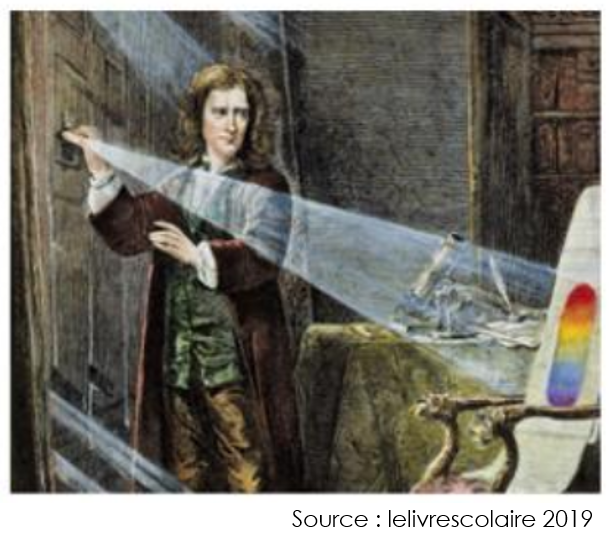
\includegraphics[width=0.4\textwidth]{Images/Isaac_Newton.PNG}
   \end{wrapfigure}
Le physicien Isaac Newton (1643-1727) a mené en 1666 une expérience sur la lumière du Soleil qui allait révolutionner la conception de l'optique que l'on avait à l'époque. Pour cela, il a réalisé une petite ouverture dans son volet afin qu'un fin faisceau lumineux pénètre dans la pièce. Il a alors placé un prisme de verre sur le trajet de la lumière. Il a constaté que la lumière était déviée par le prisme et qu'elle formait sur un écran un dégradé de couleurs allant du rouge au violet, appelé \textcolor{red}{spectre}.\\

\problematique{Quel phénomène permet d'expliquer l'apparition d'un arc-en-ciel ?}
\end{tcolorbox}

\begin{mdframed}[style=autreexo]
\textbf{\bsc{Liste du matériel}}
\begin{multicols}{2}
    \begin{itemize}
    \item Un générateur de tension continue ;
    \item Une lampe à incandescence ;
    \item Une lentille convergente ;
    \item Une fente ;
    \item Un prisme ;
    \item Un écran ;
    \item Une lampe à vapeur de mercure ;
    \item Un filtre rouge et un filtre bleu ;
\end{itemize}
\end{multicols}
\end{mdframed}

\begin{large}
    \textbf{\textcolor{red}{\underline{Travail à réaliser (20min):}}}
\end{large}
\\
\question{Au bureau, la même expérience qu'Isaac Newton a été réalisée. Observe-t'on le même résultat que le physicien ?}{Oui on observe bien le même résultat que le physicien à savoir l'apparition du spectre de la lumière blache.}{0}
\\
\question{Réaliser un schéma de l'expérience en reproduisant le résultat obtenu. On utilisera bien le vocabulaire appris dans le cours (rayon incident, réfléchi, réfracté).}{\begin{center}
    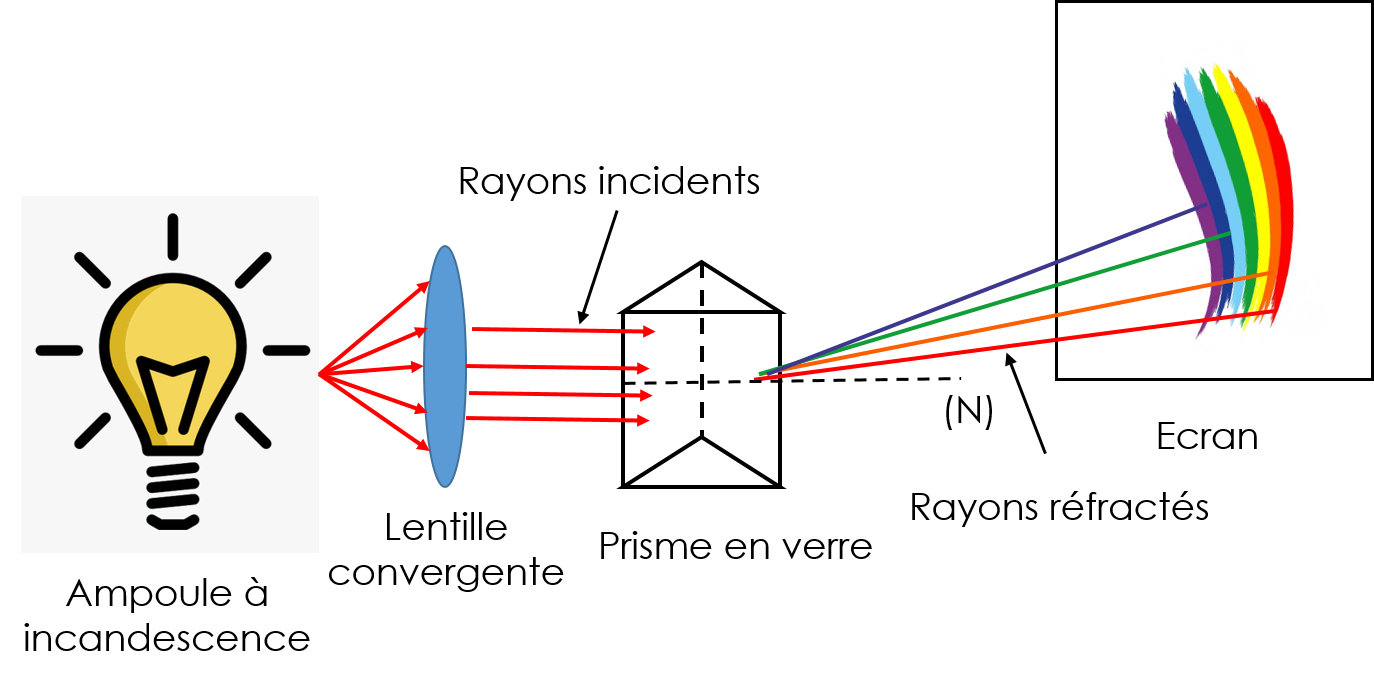
\includegraphics[scale=0.6]{Images/Montage.png}
\end{center}}{0}
%\\
\question{On définit l'angle de déviation comme l'angle entre le rayon arrivant sur le prisme et le rayon réfracté à la sortie du prisme. Indiquer quelle radiation est la plus déviée et laquelle est la moins déviée par le prisme.}{En regardant le schéma, on peut voir que le rayon violet est celui le plus dévié et le rouge est celui le moins dévié.}{0}
\\
%\question{Mettre un filtre rouge devant la sortie de la lampe à incandescence. Réaliser la même expérience avec un filtre bleu. Reproduire le résultat sur un schéma pour chacune des expériences. En déduire l'utilité d'un filtre.}{}{0}
%\\
\question{On remplace la lampe à incandescence par la lampe à vapeur de mercure. Indiquer la différence avec le spectre obtenu dans l'expérience précédente.}{\begin{center}
    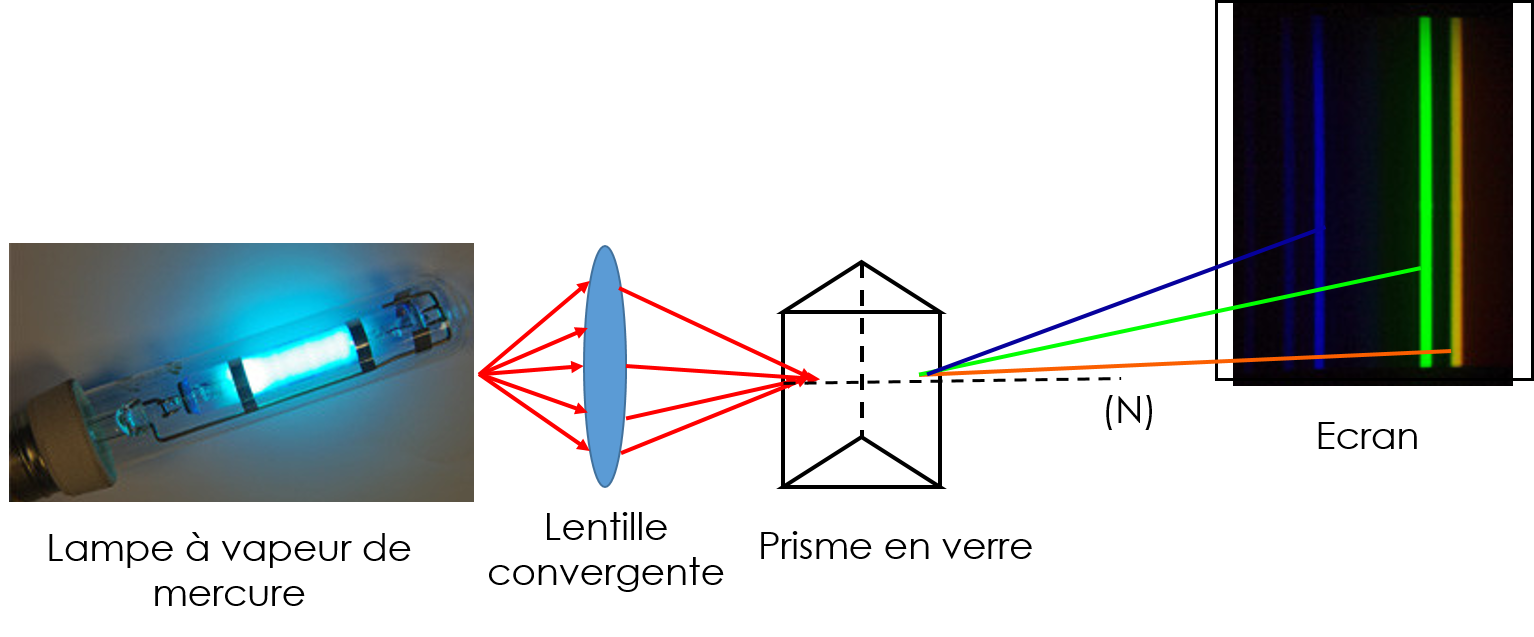
\includegraphics[scale=0.6]{Images/Montage_mercure.png}
\end{center}
On voit qu'il y a moins de couleurs dans le spectre de la lampe à vapeur de mercure que dans le spectre de la lumière blanche.}{0}
%%%% documents

\begin{center}
    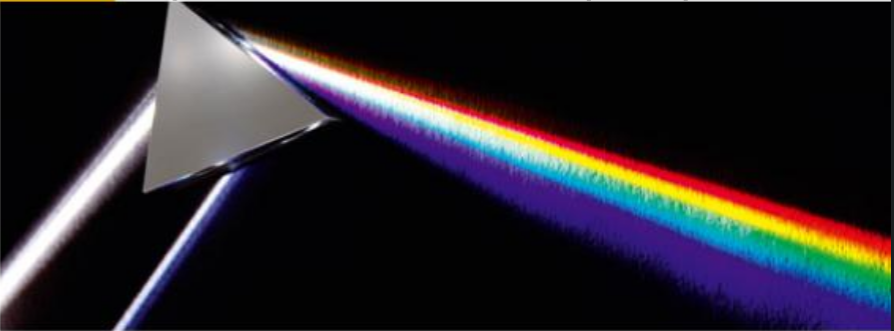
\includegraphics[scale=1.1]{Images/Dispersion.PNG}
\end{center}

%%%%
%\newpage
\section{Interprétation des résultats}

\begin{doc}{Variation de l'indice optique du verre en fonction de la radiation qui le traverse}
    L'indice optique du verre dépend de la longueur d'onde de la radiation qui le traverse : un verre est un milieu dit \textcolor{red}{dispersif}. Par exemple, pour une radiation rouge, l'indice optique $n_{rouge}=1,510$ et pour une radiation bleue $n_{bleu}=1,520$.
\end{doc}
\begin{large}
    \textbf{\textcolor{red}{\underline{Travail à réaliser (30min):}}}
\end{large}
\\
%\\
\question{Voici un prisme dont l'angle au sommet A vaut 35$\degree$ :
\begin{center}
    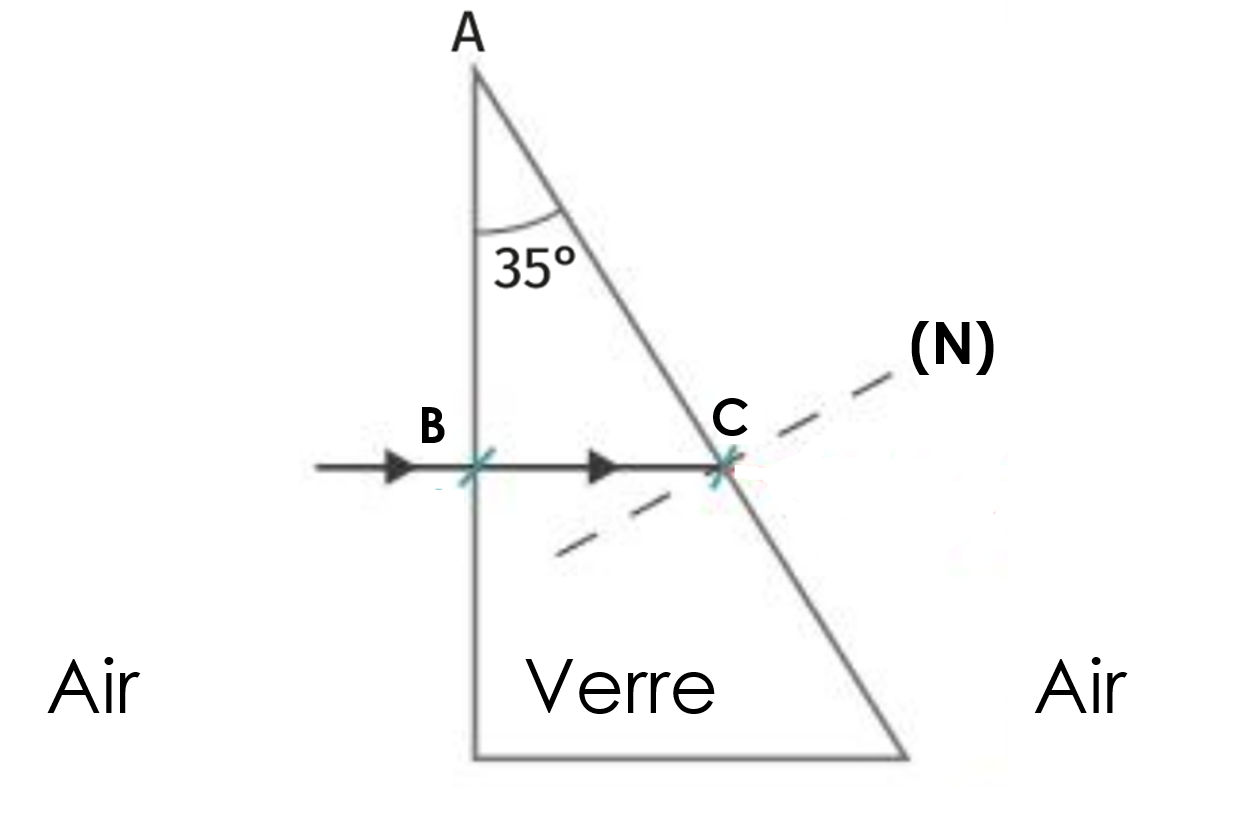
\includegraphics[scale=0.6]{Images/Prisme_exo.PNG}
\end{center}
Tracer le rayon réfléchi à l'interface verre-air (c'est-à-dire  au point \textbf{C}). Indiquer sur le schéma l'angle d'incidence $i_1$ et l'angle de réflexion $r$ en ce point.}{\begin{center}
    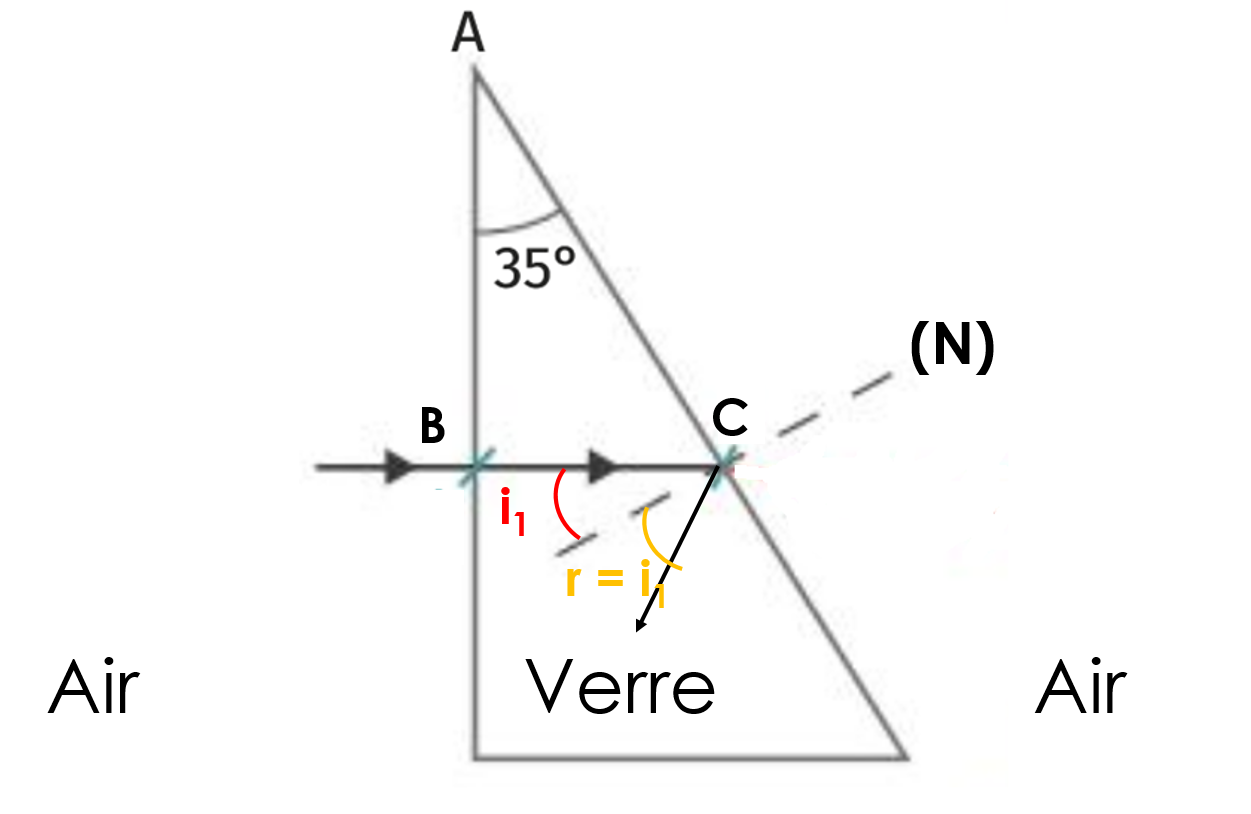
\includegraphics[scale=0.6]{Images/Prisme_correction5.png}
\end{center}}{0}
%\\
%\begin{minipage}{0.47\textwidth}

\begin{facile}{Parcours dispersion}

\question{Rappeler la loi de Snell-Descartes pour la réfraction.}{Les rayons incident et réfracté appartiennent au même plan appelé plan d'incidence. Ces deux rayons sont tels qu'on a la relation : 
\begin{equation*}
    n_1\times \sin\left(i_1\right) = n_2\times \sin\left(i_2\right)
\end{equation*}}{0}
%\\
\question{Justifier que le rayon n'est pas dévié au point \textbf{B}.}{L'angle d'incidence au point \textbf{B} vaut $0\degree$, l'angle de réfraction est donc nul d'après la loi de Descartes sur la réfraction :
\begin{equation*}
    n_{verre}\sin(0) = 0 = n_{air}\sin(i_2)
\end{equation*}
Donc $\sin(i_2)=0$ donc  $i_2=0$.}{0}
\\
\question{Déterminer l'angle de réfraction de la lumière bleue en sachant que l'angle d'incidence au point \textbf{C} vaut 35$\degree$.}{D'après la loi de Descartes sur la réfraction :
\begin{equation*}
    n_{\text{bleu}}\times \sin\left(i_1\right) = n_{air}\times \sin\left(i_{2,\text{bleu}}\right)
\end{equation*}
On en déduit que : 
\begin{equation*}
    \sin\left(i_{2,\text{bleu}}\right) = \frac{n_{\text{bleu}}}{n_{air}}\times \sin\left(i_1\right)
\end{equation*}
Et donc que : 
\begin{align*}
    i_{2,\text{bleu}} &= \arcsin\left(\frac{n_{\text{bleu}}}{n_{air}}\times \sin\left(i_1\right) \right) \\
     i_{2,\text{bleu}} &= \arcsin\left(\frac{1,520}{1,00}\times \sin\left(35\degree\right) \right) \\
     i_{2,\text{bleu}} &= 60,7\degree
\end{align*}}{0}
%\\
\question{Tracer le rayon bleu en indiquant l'angle de réfraction $i_{2,bleu}$ sur le schéma.}{\begin{center}
    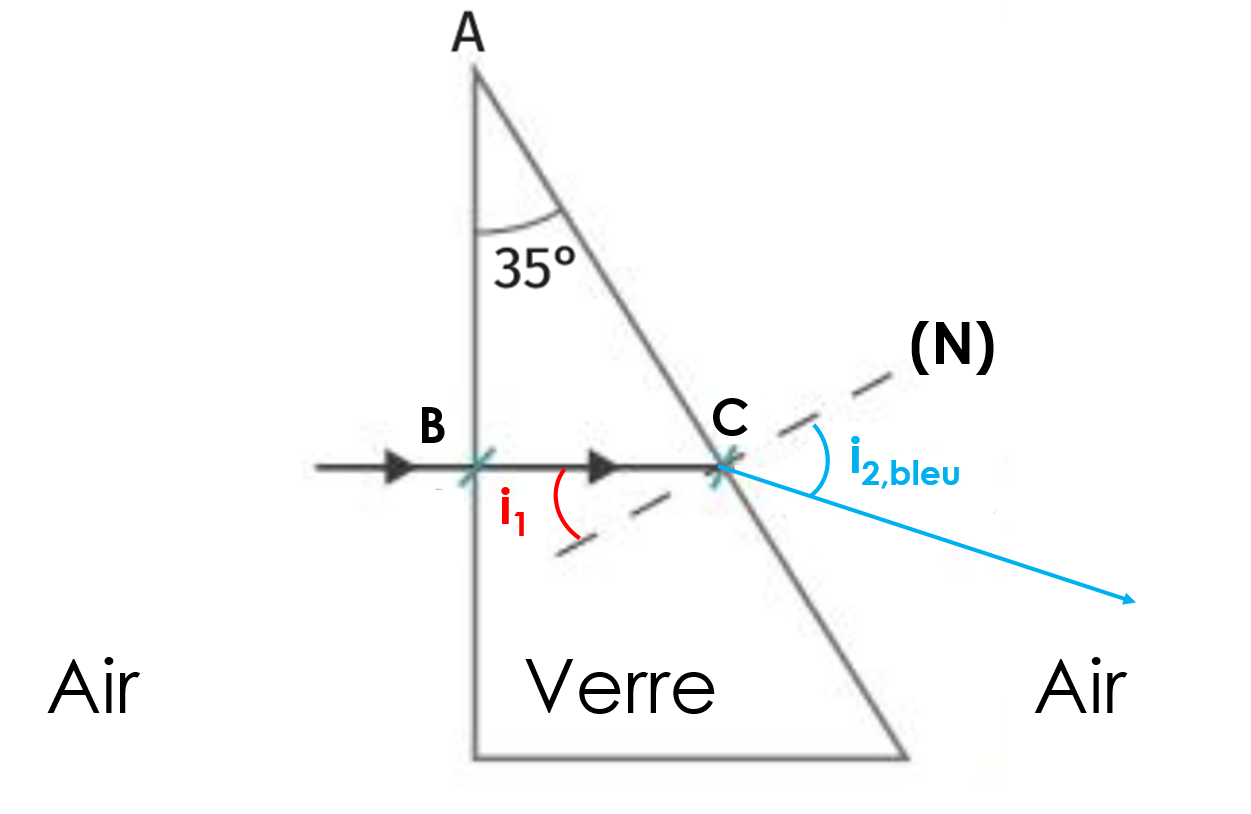
\includegraphics[scale=0.6]{Images/Prisme_correction6.png}
\end{center}}{0}

\end{facile}
%\end{minipage}
%
%\hspace{0.05\textwidth}
%\begin{minipage}{0.47\textwidth}
%\vspace{-2.5cm}

\begin{difficile}{Parcours Newton}
\question{Tracer les rayons rouge et bleu en indiquant précisément les angles de réfraction $i_{2,rouge}$ et $i_{2,bleu}$. Justifier chaque étape de calcul.}{Merci à Gabrielle Reniez et Laura Leung pour cette très belle démonstration ! 
\begin{center}
    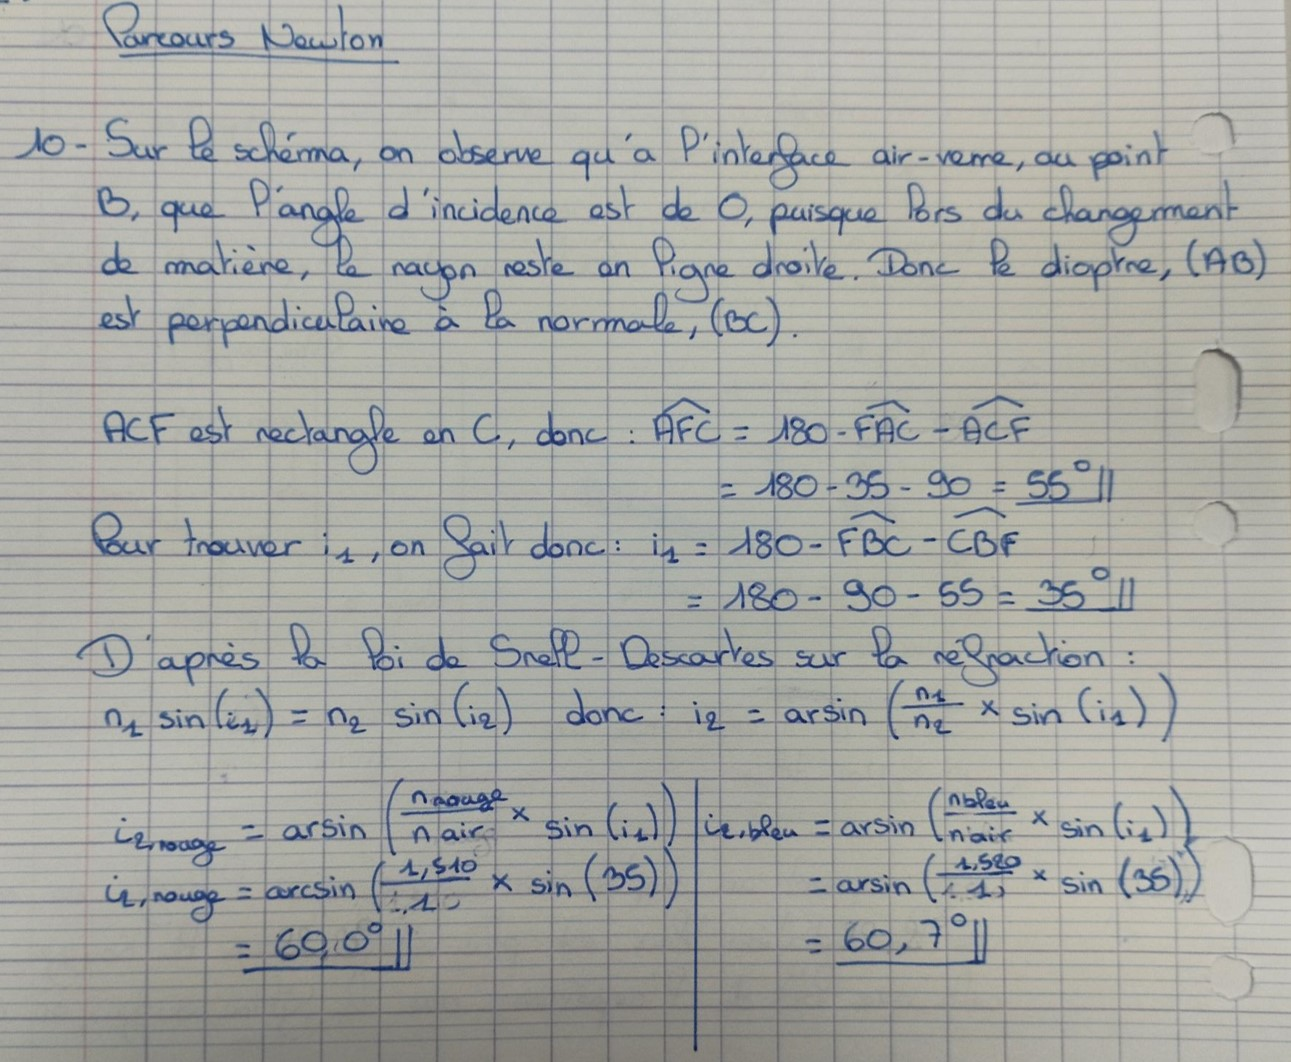
\includegraphics[scale=0.7]{Images/Correction_Newton.jpg}
\end{center}
On peut alors tracer les rayons bleu et rouge :
\begin{center}
    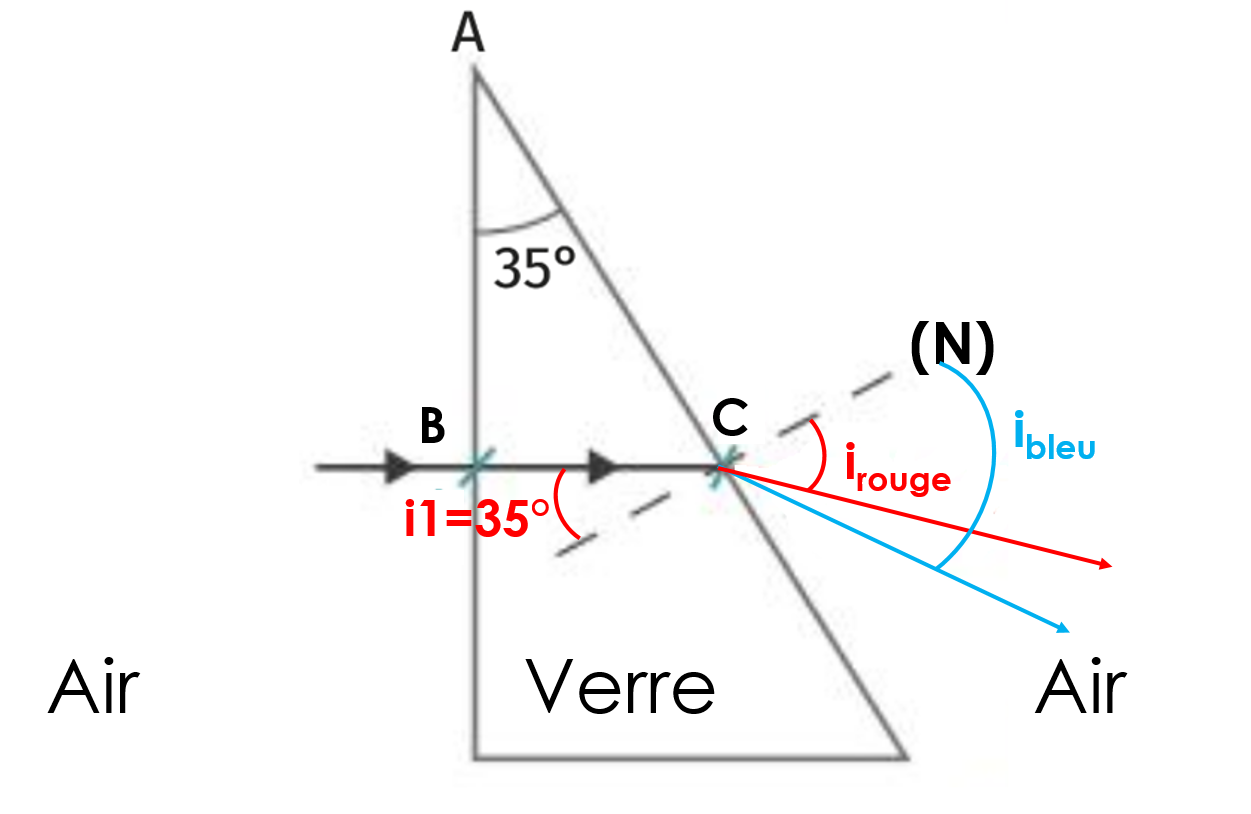
\includegraphics[scale=0.6]{Images/Prisme_correction10.png}
\end{center}}{0}
\end{difficile}
\hfill
%\end{minipage}

%\newpage

\begin{difficile}{\large Bilan de l'activité sur la dispersion}
\vspace{0.5cm}
\question{Quel phénomène permet d'expliquer la déviation de la lumière par le prisme ?}{Il s'agit de la réfraction. Celle-ci dépend de la longueur d'onde (la couleur autrement dit) de la lumière. Lorsque l'indice optique d'un milieu dépend de la longueur d'onde, on dit que le milieu est \underline{dispersif}.}{0}
\\
\question{Lors de la formation d'un arc-en-ciel, quel élément joue le rôle de prisme ?}{Il s'agit des gouttes d'eau composant la pluie.}{0}
    \texteTrouMultiLignes{~}{15}
\end{difficile}
%\newpage
%\papiermillimetre